\documentclass{article}
\usepackage[utf8]{inputenc}
\usepackage[margin=1in]{geometry}
\usepackage{graphicx}
\usepackage{hyperref}
\hypersetup{
    colorlinks=true,
    linkcolor=blue,
    filecolor=magenta,
    urlcolor=black,
}
\newcommand{\n}{\noindent}

\begin{document}
\title{Sudo rm -rf / \\ \large{Politifind}}
\author{Fall 2017}
\date{}
\maketitle

\n\textbf{Overview}:\\

\n\textbf{Members}: Andrew Bass, Matthew Bissaillon, Matthew Gramigna, Justin Kennedy \\

\n\textbf{Github}: \url{https://github.com/arbass22/politifind} \\

\n\textbf{User Interface}: Must make sure to pip install algoliasearch\_django\\

\n\textbf{Data Model}: The following diagram is our updated data model for Politifind with the following descriptions: \\ 

\n\textit{Profile}: Includes authentication fields for the django User as well as information about this user's politifind profile. \\
\n\textit{Politician}: Represents a member of congress in either the house or senate. \\
\n\textit{Bill}: A congressional bill.\\
\n\textit{PoliticianVote}: Indicates how a specific Politician voted on a specific bill. \\
\n\textit{UserVote}: Indicates how a specific politifind user voted on a specific bill.\\
\n\textit{Committee}: Represents a committee in congress. \\
\n\textit{SubCommittee}: Represents a subcommittee of an existing politifind Committee object. \\
\n\textit{CommitteeMembership}: Indicates that a specific Politician is a member of a specific Committee. \\
\n\textit{BillCommittee}: Indicates that a specific Committee introduced a specific Bill. \\
\n\textit{BillSponsorship}: Indicates which Politician sponsored a specific Bill. \\
\n\textit{BillAction}: An action that has happened on a specific Bill. \\
\n\textit{UserPoliticianSubscription}: Indicates that a politifind user subscribed to a specific Politician. \\
\n\textit{UserBillSubscription}: Indicates that a politifind user subscribed to a specific Bill.\\
\n\textit{UserCommitteeSubscription}: Indicates that a politifind user subscribed to a specific Committee.\\

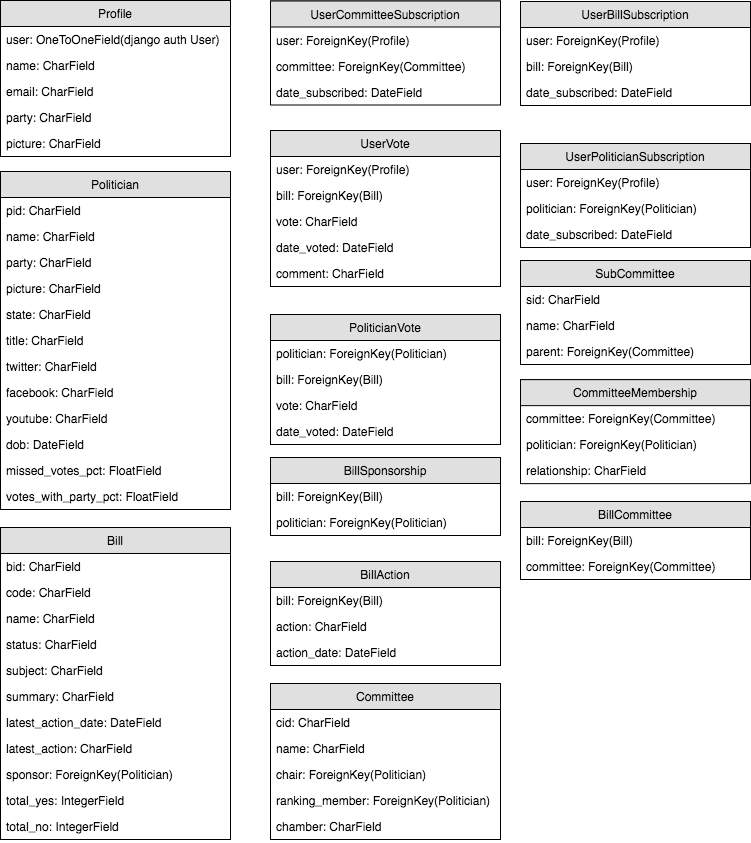
\includegraphics[scale=0.5]{politifind-data-model-UPDATED.png} \\

\n\textbf{URL Routes/Mappings}: 
\begin{center}
\begin{tabular}{ l | l | l }
route & name & description \\
\hline
r`\^{}\$' & index & route users to the home page \\
r`\^{}bill/(.*)/\$' & bill & individual bill page\\
r`\^{}politician/(.*)/(bills$\mid$votes)*' & politician & individual politician page\\
r`\^{}politicians/\$' & politicians & list of all politicians\\
r`\^{}bills/\$' & bills & list of all bills\\
r`\^{}committee/(.*)/(bills$\mid$subcomittees)*\$' & committee & individual committee page\\
r`\^{}committees/\$' & committees & list of all committees\\
r`\^{}profile/\$' & profile & user's profile page\\
r`\^{}search/\$' & search & display's search results\\
r`\^{}accounts/' & accounts & adds login/logout/etc urls\\
r`\^{}vote/(.*)/(yay$\mid$nay)*/' & vote & view individual vote page\\
r`\^{}subscribe/\$' & subscribe & user can subscribe\\
r`\^{}unsubscribe/\$' & unsubscribe & user can unsubscribe\\
r`\^{}profile/update/' & update profile & have a user update their profile page\\
\end{tabular}
\end{center}
\\

\n\textbf{Authentication/Authorization}: \\

\n\textbf{Team Choice}: \\

\n\textbf{Conclusion}: \\

\end{document}
